%
We will start the introduction by giving a motivation to the work done in this thesis by putting the thesis in a larger context, and is meant for an audience with only basic knowledge of physics.
At the end of the chapter, an outline of the structure of the thesis will be given.

\section{Motivation}
%
The ultimate motivation of this thesis is set by providing clean energy%
\footnote{Words like "energy consumption" will here be referring to conversion of energy in a low entropy state to the same amount of energy in a higher entropy state.
}
%
to a growing population with an increasing standard of living.
One projection of the increased energy demand is given in \cref{fig:energyDemand}.
%
\begin{figure}[htb]
    \begin{center}
        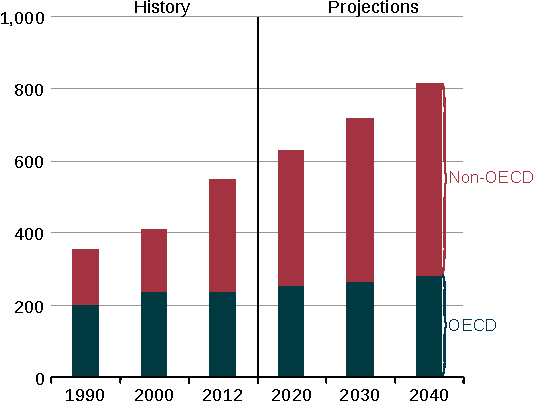
\includegraphics{fig/intro/energyDemand}
    \end{center}
    \caption{Historic and projected energy consumption from \cite{UEIA2016book}.
    The ordinate is given in quadrillion British thermal unit, which approximately equals $10^{18} \J$.
    }
    \label{fig:energyDemand}
\end{figure}

\noindent
As the bulk-part of the current energy consumption is provided by limited energy sources, a more sustainable approach is needed.

One candidate for a more sustainable energy production is through thermonuclear fusion.
We will here give a short summary of the process.
For more introduction on the topic, see \cite{Freidberg2008book}.
If two nuclei can overcome the electrostatic Coulomb-barrier (with the "help" of quantum tunneling), they can fuse into a heavier nucleus.
The process will release a surplus of energy if the mass of the resulting nucleus is lighter than the sum of the two initial nuclei.
The main reaction sought is the $\text{D}-\text{T}$ reaction, which can be summarized as
%
\begin{align*}
    \text{D} + \text{T} \to \text{He}^4 + \text{n} + 17.6 \text{MeV},
\end{align*}
%
where the deuterium $\text{D}$ can be distilled from sea water, whereas the tritium $\text{T}$ must be produce due to scarce availability and a short half-life of $12.3$ years.
Probably the easiest way to obtain $\text{T}$ is by breeding it from lithium through the process
%
\begin{align*}
    \text{Li}^6 + \text{n} &\to \text{T} + \text{He}^4 + 4.8 \text{MeV}\\
    \text{Li}^7 + \text{n} &\to \text{T} + \text{He}^4 + \text{n} - 2.5 \text{MeV}.
\end{align*}
%
The need of $\text{Li}$ could theoretically be replaced by tritium breeding from the $\text{D}-\text{D}$ reaction
%
\begin{align*}
    \text{D} + \text{D} \to \text{T} + \text{p} + 4.03 \text{MeV}.
\end{align*}
%

However, this is a much harder reaction to achieve, as it requires substantially higher temperatures.

Man made thermonuclear fusion delivering energy on the grid has yet to be achieved.
It is still unclear whether or not man made thermonuclear fusion can be produced in technological and scientifically feasible way.
The ITER \cite{ITERWeb} project, which has a first plasma operation currently planned in $2025$, is meant to give a better answer to this question by yielding a tenfold energy output compared to the energy input.
The goal of ITER is not to supply the grid with energy.
This is planned to be done by the prototype fusion reactor DEMO, which is still in the planning phase, and is meant to answer questions about economically viability.
Scientific and economical feasibility aside, the potential benefits and sustainability of fusion energy is great.
To illustrate this let's look at some very approximated numbers, only to get an idea of what ballpark we are in.
We can assume that on average a UK citizen uses $195 \text{\;kWh}$ per day%
\footnote{As a comparison to this, MacKay makes an optimistic estimate that UK could yield $180 \text{\;kWh}$ per person per day from current day technology renewables in \cite{Mackay2009book}}%
%
\cite{Mackay2009book}.
If we now assume a population $12$ billion people \cite{Melorose2015}, and that the average consumption per person is $195 \text{\;kWh}$ per day, we can make a crude estimate on how long the fusion resources will last.
The estimate is show in \cref{fig:potFusion}.
%
\begin{figure}[htb]
    \begin{center}
        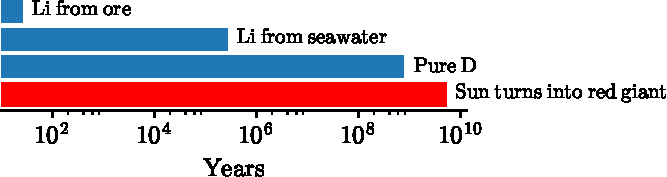
\includegraphics{fig/intro/fusionSustain}
    \end{center}
    \caption{Estimated years one could power the world on fusion with a population of $12$ billion people using in average $195 \text{\;kWh}$ per day.
        It is assumd that all available $\text{Li}$ is used for fusion based on the $\text{D}-\text{T}$ reaction, and that all available $\text{D}$ is used for the for fusion based on the $\text{D}-\text{D}$ reaction.
        With the approximated numbers obtained from \cite{Melorose2015,Mackay2009book,ongena2012,Eckhartt1995}.}
    \label{fig:potFusion}
\end{figure}

Many of the challenges fusion is facing can be summarized with the following quote by Sebastien Balibar \cite{Balibar2009Web}:
%
\begin{quote}
    Fusion is like trying to put the Sun in a box - but we don't know how to make the box.
\end{quote}
%
As the plasma in a working reactor will be held at temperatures at several $10 \keV$ (which translates to several $100$ million Kelvin), conventional materials can not be used as a "box".
Instead, as the plasma will be in an ionized state, the plasma can be kept in place using a strong magnetic field, as each individual particle of species $\a$ is subjected to the Lorentz force
%
\begin{align*}
    \ve{F}_\a = q_\a \L(\ve{E} + \ve{v}_\a\times\ve{B}\R),
\end{align*}
%
and will therefore (at least to first order) move freely parallel to the magnetic field, but be locked to a magnetic field in the perpendicular direction.
Thus, the "box" which until now has proven most successful%
\footnote{Alternative concepts such as the "stellarator" and the "spherical tokamak" are areas of active research, and could turn out to serve as better options for the "box" in the future.}
%
, and which ITER will be based on, is the tokamak, depicted in \cref{fig:tokamak}.
%
\begin{figure}[htb]
    \begin{center}
        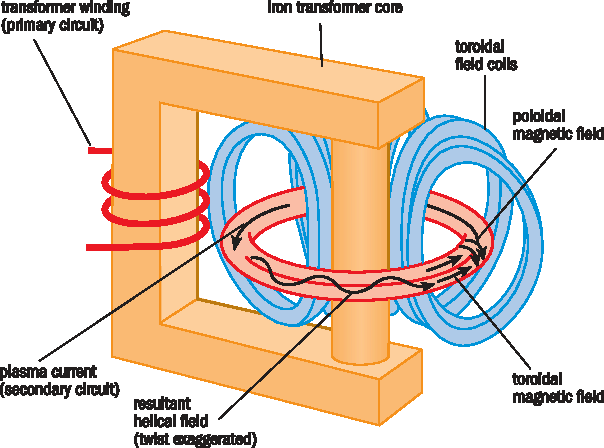
\includegraphics{fig/intro/tokamak}
    \end{center}
    \caption{Simplified schematics of the tokamak from \cite{nuttall2008}.
        A more detailed view of the ITER tokamak can be found in \cite{ITERWeb}.}
    \label{fig:tokamak}
\end{figure}

In the tokamak a twisted, closed magnetic field in a toroidal configuration is used to keep the plasma in place.
Close to the toroidal axis the magnetic field closes itself
%
\footnote{Possibly after an infinite number of toroidal revolutions.}
%
without intersecting with the materials of the tokamak, spanning a magnetic surface.
These field lines are referred to as "closed" field lines.
Moving radially outwards from the toroidal axis the magnetic field is no longer closing only on itself, but rather through a material surface.
These field lines are referred to as "open" field lines.
In order to remove impurity production and plasma recycling away from the main plasma, the open field lines are diverted away from the main plasma to divertor plates%
%
\footnote{Diverting the plasma has a lot of other benefits as described in detail in \cite{Stangeby2000book,Stacey2012book}.}%
%
.
Thus when moving radially, the plasma is transitioning from the \emph{plasma edge}, through the position of the \emph{Last Closed Field Surface} LCFS to the region of open field lines called the \emph{Scrape-Off Layer} (SOL).
Since the plasma particle motion is constrained in the radial direction through gyration, large pressure gradients develops around the LCFS.
Instabilities in the edge region can develop from these gradients, both on the macroscopic (machine size) scale in form of ELMs \cite{Zohm1996}, but also on the microscopic scale (usually in the order of $\mm - \cm$) such as interchange instabilities \cite{Scott2005b} and drift-waves \cite{Tynan2009}.
These microscopic instabilites develops into turbulence, and this turbulence is believed to be the cause of the increased transport levels
%
\footnote{In the so called H-mode this turbulent transport can be suppressed down to the neoclassical levels by a strong shear flow \cite{Burrell1997}.}%
%
which exceeds those predicted by \emph{classical} transport from colliding particles, and those predicted by neoclassical theory (which includes transport effect arising from the magnetic field geometry) \cite{Wootton1990}.

Although advances has been done in the last decades, the turbulent processes in the edge and SOL is still not fully understood.
There are for example a lot of open questions related to coherent structures called \emph{blobs} which emerges from the turbulence \cite{DIppolito2011}.
In other words, the "box" is "leaking", and we would like a better understanding of how and why it is leaking.
The success of ITER achieving a high energy gain would be bleak if it turns out that part of the divertor got melted due to unforeseen turbulent events.

The turbulent processes in the edge and SOL of a tokamak is hard to analyze, as several physical processes can be active at once.
If one can get a good overview of the individual physical processes first, studying the full system will become easier.
An additional challenge is to measure the processes around the LCFS in a tokamak due the high temperature and due to the difficulties to properly resolve the spatial and temporal scales with few measuring points.
Both these obstacles can be reduced by analyzing processes similar to those found in around the LCFS in a linear machine.
In such a machine, the interchange instability can be eliminated if the machine operates with a straight magnetic field.
The temperatures is also lower in a linear machine, which makes plasma measurements easier.
Hence, they are beneficial for benchmarking numerical codes.
Linear machines can usually be operated so that the plasma is freely streaming towards a material surface, which is similar to the situation found in the SOL where the plasma is diverted to the divertor plates with help of the magnetic fields.

This brings us to the aim of this thesis:
To numerically simulate some of the processes taking place in a linear machine in order to gain insight in non-curvature driven instabilities.
Linear machines in themselves are interesting for fusion research and is besides turbulent studies used for material testing \cite{Rapp2010}, studies of \emph{magnetic reconnection} with \emph{X-points} \cite{Bohlin2014} and studies of \emph{plasma detachment} \cite{Ohno2017} to mention some.
We will however limit the scope of this thesis to include only turbulent processes in a straight magnetic field.

Next, let us also state how accurate we would like to be when investigating the plasma.
One could say that one want the investigation to be $100 \%$ accurate, and include all known physic in the investigation, following the quantum mechanical wave-function of each particle as a function of time.
Although tempting, it is easy to show that such a task is not feasible with the current computer technologies.
Imagine just to assign a number to each particle in a $1\m^3$ box with a particle density of $10^{18} \m^{-3}$ particles%
\footnote{These are approximately the particle numbers we will work with in this thesis.}%
%
using $4$ bytes.
This would require $4$ exabytes of storage.
Therefore, we seek to simplify the system while still retaining the important details.
The task is comparable to investigate the time it takes a white ball takes to fall.
Does it matter that the ball is white?
One could imagine that there are some reflection properties of the white ball which alters the fall-time.
However, such an effect would most likely be negligible.
The fact that the ball is white would be far more relevant if we would like to find the cooling time of the ball.

Therefore, instead of following every single particle, we will make some averages on the system which gives us a fluid like description of the plasma.
We will further simplify the system by investigating which terms in our model which is small compared to the rest of the terms.
This gives us a model which we be can used to investigate physics happening at a slower scale than the frequency the ions gyrates around the magnetic field line (which in our linear machine is a couple of hundred $\kHz$), and spatial scale around the ion gyration radius taken at the electron temperature (which in our case is around a $\cm$).
Notice that we by doing so have excluded physical processes like propagation of electromagnetic waves through the plasma.
Although out of scope of our investigation, such a process is important when for example looking at heating of the plasma using electromagnetic waves.
We will in our model use a global approach, meaning that we will model the entire plasma, rather than the traditional approach where only fluctuations are investigated.

As such, this thesis does not answer ultimate questions such as:
"How can the plasma be operated in order to make man made fusion energy be economically viable."
Rather, this thesis makes a very humble contribution needed to answer such questions.
More precisely, this thesis aims to answer the following questions:
%
\begin{itemize}[noitemsep]
    \item What model is suitable for modeling the low frequency turbulence observed in a linear machine?
    \item What numerical approaches can be used for solving our model?
    \item How is the plasma evolving in a linear machine?
    \item To what extent does the approximation know as the Boussinesq-approximation, which is often done, alter the solution?
    \item Can coherent structures as blobs and holes be found from our model?
% FIXME: Check that this is fulfilled
    \item Are zonal flows found in our model?
    \item Does our model capture the features reported in the literature?
\end{itemize}



\section{Thesis structure}
%
The remainder of this thesis is structured into $6$ main-parts.

As we would like to simulate a set of equation derived more or less from first principles, the \cref{part:CELMA} is dedicated to the derivation of the CELMA model.
To enable full transparency of the derivation, most intermediate calculation step are also shown.
As such, this thesis is addressed to a readership familiar with basic concepts of plasma physics.
Readers familiar with these derivations may readily skip these intermediate steps, but should pay extra attention to the derivation of the modified vorticity equation, as (to the authors best knowledge) this is not given elsewhere.
In \cref{chap:kin} the derivation of the fluid equations is done by taking moments of the Fokker-Planck equation including a particle source.
The first two fluid moments is taken, and the fluid closure is done by assuming a constant temperature.
These equations are further refined using the drift-fluid approximation in \cref{chap:drift-order}, where also the fluid drifts are given.
In \cref{chap:slowB} we restrict the system to only be valid for a slowly varying $B$-field, whereas in chapter \cref{chap:CELMA} a straigth magnetic field in a cylinder geometry is imposed.
The boundary conditions of the model is also given in \cref{chap:CELMA}.
The alternative model, which uses the Boussinesq approximation is given in chapter \cref{chap:boussinesq} before \cref{part:CELMA} is concluded by a summary.

In \cref{part:impl} all the details of the numerical implementation is given.
\Cref{chap:implBOUT++} describes the built-in options from the BOUT++ framework which is used in this thesis, and is followed by implementations which are not included in the BOUT++ in \cref{chap:additionalImplementation}.
The verification of the numerical implementation is given in \cref{chap:verification}.

Finally, the results from the numerical simulations are given in \cref{part:results}.
The setup is briefly given in \cref{chap:setup}, followed by a description of the phases of the model in chronological order.
\Cref{chap:ss} describes the steady state found from the simulations.
The system is perturbed and the following linear state is described in \cref{chap:linear} together with simplified linear drift wave theory.
The resulting turbulent state is presented in \cref{chap:satTurb}, and the characteristic of the fluctuation is given in \cref{chap:charTurb}.
% FIXME
FIXME \cref{chap:zonal} not given.
Investigation of how the system scales with varying $B$-field strength is given in \cref{chap:BFScan}, and the comparison with the model using Boussinesq approximation is given in \cref{chap:compBouss}.
% FIXME
FIXME \cref{chap:neutScan} not given.

A summary of the conclusion and outlook of this thesis is given in \cref{part:concl}.

To supplement, appendices are given in \cref{part:app}. These appendices are being referred to throughout the text with exception of \cref{app:shortcomings} which summarizes the shortcomings in this thesis.
